 \documentclass[a4paper,10pt]{article}
\input{/Users/WannaGetHigh/workspace/latex/macros.tex}

\title{Rapport TP1 : SMA - Billes}
\author{Fran\c{c}ois \bsc{Lepan} - Alexis \bsc{Linke}}

\begin{document}
\maketitle

\section{Choix}

Nous sommes partis sur un syst\`eme de d\'eplacement sur une grille case par case. Deux agents ne peuvent  se retrouver sur une m\^eme case.

Nous avons fait ce choix car le syst\`eme de collision ainsi que la repr\'esentation sur un \verb&JPanel& est plus facile \`a g\'erer qu'un syst\`eme de d\'eplacement libre.

Les couleurs des agents sont fix\'es lors de leurs cr\'eation.

\section{UML + explication}

\begin{figure}[ht]
\begin{center}
	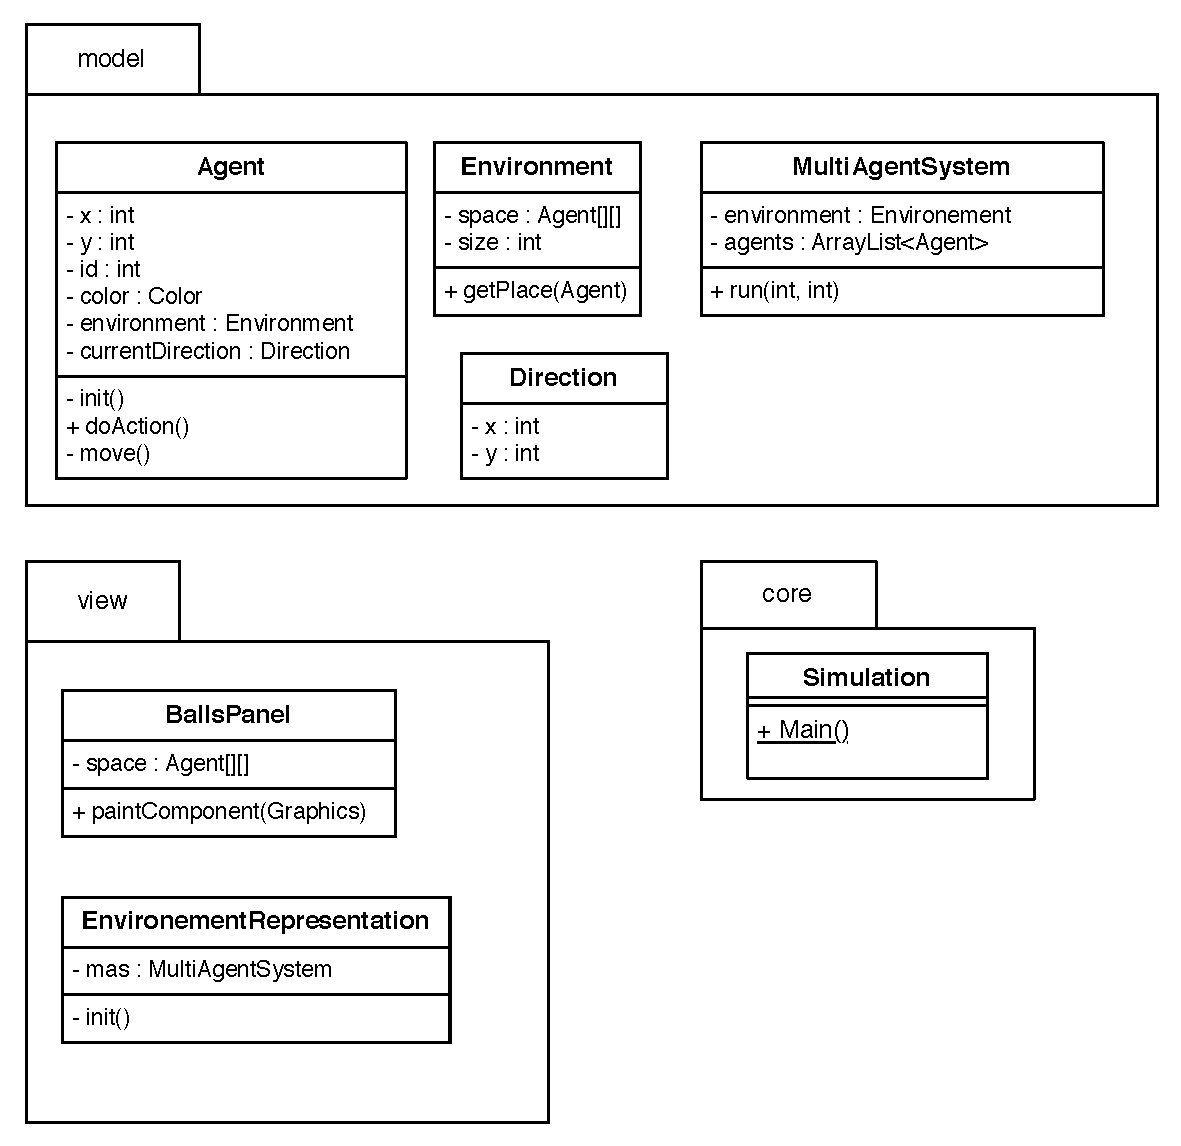
\includegraphics[height=9.3cm , width=11cm]{uml/sci_uml_tp1.pdf}
\end{center}
	\caption{UML}
	\label{uml}
\end{figure}

\newpage 

Le design pattern utilis\'e pour r\'ealiser ce programme est le MVC.  Il y a 3 packages : \emph{core}, \emph{view} et \emph{model}. 

Le package \emph{core} contient la classe principale \verb&Simulation& qui ex\'ecute le programme. 

Ensuite le package \emph{view} contient les classes \verb&BallsPanel& qui repr\'esente le panel sur lequel on dessine les billes et \verb&EnvironmentRepresentation& qui est la \emph{vue} du MVC ainsi que la fen\`etre dans laquelle on ajoute le panel \verb&BallsPanel&. 

Et enfin on a le package \emph{model} qui lui contient toutes les classes n\'ecessaire aux calcules de collisions ainsi que de position tout au long de l'ex\'ecution du programme. La classe \verb&Agent& contient les donn\'ees n\'ecessaires pour situer et identifier un agent au sein de l'environnement. La classe \verb&Environment& contient une grille d'\verb&Agent& et poss\`ede une m\'ethode \verb&getPlace(Agent)& qui permet d'allouer une place sur cette grille qui est utilis\'e lors de l'ajout d'un agent dans la classe \verb&MultiAgentSystem&. Cette classe est le \emph{model}. Elle contient une liste d'\verb&Agent& ainsi que l'\verb&Environment& dans lequel les agents se meuvent et la m\'ethode \verb&run()& qui \`a chaque tour donne la parole \`a chaque agents de fa\c{c}on \'equitable.
 
\section{Compilation + fonctionnement}
 
\paragraph{Compilation} ~\\
Se mettre dans le dossier src $\rightarrow$ \verb&javac core/Simulation.java&

\paragraph{Execution} ~\\
Ne pas bouger du dossier src \\
\verb&java core.Simulation <taille> <nb agent> <nb tour> <delai entre chaque tour>& \\
Si on rentre un nombre de tour = -1 alors c'est infini

\paragraph{Exemples} ~\\
\verb&java core.Simulation 100 50 -1 5& \\
\verb&java core.Simulation 10 5 100 5& \\
\verb&java core.Simulation 50 40 -1 5& \\

\section{Probl\`eme}

Nous avons un probl\`eme pour le redimensionnement de la fen\`etre, il y a un e\'cart qui se forme en bas et \`a droite de cette fen\`etre

\end{document}